\documentclass[11pt]{article}
\usepackage[T1]{fontenc}
\usepackage[utf8]{inputenc}
\usepackage[polish]{babel}
\usepackage{amsthm}
\usepackage{amsmath}
\usepackage{program}
\usepackage{amsfonts}
\usepackage{titlesec}
\usepackage{graphicx}
\title{%
  Sprawozdanie \\
  \large P3.20 z analizy numerycznej\\
    Obliczanie $A^{-1}$ za pomocą rozkładu QR macierzy}
\author{Artur Derechowski\\Mateusz Markiewicz}
\begin{document}
\maketitle
\tableofcontents

\newtheorem{definition}{Definicja}[section]

\titleformat{\paragraph}
{\normalfont\normalsize\bfseries}{\theparagraph}{1em}{}
\titlespacing*{\paragraph}
{0pt}{3.25ex plus 1ex minus .2ex}{1.5ex plus .2ex}

%~~~~~~~~~~~~~~~~~~~~~~~~~~~~~~~~~~~~~~~~
\section{Wstęp}
Macierzą odwrotną do $A$ nazywamy macierz $A^{-1}$ taką, że $AA^{-1} = A^{-1}A = I$. Jest kilka sposobów obliczania macierzy odwrotnej. W naszej pracowni przedstawiamy dwa z nich, czyli rozkład QR i rozkład LU, a następnie porównamy obie te metody.

\subsection{Cel zadania}
Zadanie zostało podzielone na dwie części. Wyznaczamy rozkład macierzy $A = QR$, gdzie $Q$ jest
macierzą ortogonalną, a $R$ macierzą górnotrójkątną.\\
Następnie wyznaczamy również rozkład macierzy $A = LU$, gdzie $L$ i $U$ są odpowiednio macierzami
dolno i górnotrójkątnymi.\\
Następnie wykorzystujemy oba te rozkłady do policzenia macierzy odwrotnej do $A$ i badamy je pod względem
dokładności.

\subsection{Streszczenie sprawozdania}

Po teoretycznym wprowadzeniu do omawianego zagadnienia przejdziemy do opisu metod znajdowania $A^{-1}$ opartych na rozkładach $QR$ oraz $LU$. Przedstawimy algorytmu używane w tych metodach. Następnie zajmiemy się porównaniem tych metod, zarówno w sposób teoretyczny, jak i praktyczny. Porównamy zarówno dokładność obu tych metod, jak i ich numeryczną poprawność. Na końcu przedstawimy wnioski płynące z wyników obliczeń.

\section{Opis teoretyczny problemu}
\subsection{Wprowadzenie do zagadnienia}

\textbf{Macierz} $A$ to prostokątna tablica danych jednego typu, w której każdy element numerowany jest za pomocą dwóch współrzędnych w następujący sposób:
\begin{center}
\begin{math}
A = 
\begin{bmatrix}
    a_{11} & a_{12} & \dots  & a_{1m} \\
    a_{21} & a_{22} & \dots  & a_{2m} \\
    \vdots & \vdots & \ddots & \vdots \\
    a_{n1} & a_{n2} & \dots  & a_{nm}
\end{bmatrix}
\end{math}
\end{center}
Każda kolumna tej macierzy ma $n$ elementów, a każdy wiersz $m$ elementów,\\ o takiej macierzy mówimy, że jest rozmiaru $n \times m$. Macierz, która ma tyle samo elementów w kolumnach i wierszach jest nazywana macierzą kwadratową o rozmiarze $n \times n$.

\textbf{Mnożenie macierzy} $A \cdot B$ zdefiniowane jest w następujący sposób:

\begin{center}
\begin{math}
\begin{bmatrix}
    a_{11} & a_{12} & \dots  & a_{1m} \\
    a_{21} & a_{22} & \dots  & a_{2m} \\
    \vdots & \vdots & \ddots & \vdots \\
    a_{n1} & a_{n2} & \dots  & a_{nm}
\end{bmatrix}
\cdot
\begin{bmatrix}
    b_{11} & b_{12} & \dots  & b_{1p} \\
    b_{21} & b_{22} & \dots  & b_{2p} \\
    \vdots & \vdots & \ddots & \vdots \\
    b_{m1} & b_{m2} & \dots  & b_{mp}
\end{bmatrix}
=
\begin{bmatrix}
    c_{11} & c_{12} & \dots  & c_{1p} \\
    c_{21} & c_{22} & \dots  & c_{2p} \\
    \vdots & \vdots & \ddots & \vdots \\
    c_{n1} & c_{n2} & \dots  & c_{np}
\end{bmatrix}
\end{math}
\end{center}
\begin{center}
gdzie $c_{ij} = \sum_{k=1}^{m} a_{ik} b_{kj}$
\end{center}
Warto zauważyć, że aby mnożenie macierzy $A$ i $B$ było możliwe muszą być one odpowiednich rozmiarów. Dla macierzy $A$ rozmiaru $n \times m$ macierz $B$ musi być rozmiaru $m \times p$ dla powolnego $p$. Macierz wynikowa $C$ jest wówczas rozmiaru $n \times p$.\\
Mnożenie macierzy nie jest przemienne, czyli $A \cdot B \neq B \cdot A$.

\textbf{Macierzą jednostkową} (identycznościową, tożsamościową) $I$ nazywamy macierz rozmiaru $n \times n$ zawierającą $1$ na przekątnej oraz $0$ na pozostałych współrzędnych.

\begin{center}
\begin{math}
I = 
\begin{bmatrix}
    1 & 0 & \dots & 0 \\
    0 & 1 & \dots  & 0 \\
    \vdots & \vdots & \ddots & \vdots \\
    0 & 0 & \dots  & 1
\end{bmatrix}
\end{math}
\end{center}

Dla danej macierzy $A$ określamy $A^{T}$, czyli \textbf{macierz transponowaną} macierzy $A$ w następujący sposób:
\begin{center}
\begin{math}
A^{T} = 
\begin{bmatrix}
    a_{11} & a_{12} & \dots  & a_{1m} \\
    a_{21} & a_{22} & \dots  & a_{2m} \\
    \vdots & \vdots & \ddots & \vdots \\
    a_{n1} & a_{n2} & \dots  & a_{nm}
\end{bmatrix}^{T}
=
\begin{bmatrix}
    a_{11} & a_{21} & \dots  & a_{m1} \\
    a_{12} & a_{22} & \dots  & a_{m2} \\
    \vdots & \vdots & \ddots & \vdots \\
    a_{1n} & a_{2n} & \dots  & a_{mn}
\end{bmatrix}
\end{math}
\end{center}

\textbf{Macierzą dolnotrójkątną} $L$ lub \textbf{macierzą górnotrójkątną} $U$ nazywamy macierz, której współczynniki odpowiednio nad lub pod główną przekątną wynoszą $0$.

\begin{center}
\begin{math}
L
=
\begin{bmatrix}
    l_{11} & 0  & \dots  & 0 \\
    l_{21} & l_{22} & \dots  & 0 \\
    \vdots & \vdots & \ddots & \vdots \\
    l_{n1} & l_{n2} & \dots  & l_{nn}
\end{bmatrix}
\hspace{2em} U = 
\begin{bmatrix}
    u_{11} & u_{12} & \dots  & u_{1n} \\
    0 & u_{22} & \dots  & u_{2n} \\
    \vdots & \vdots & \ddots & \vdots \\
    0 & 0 & \dots  & u_{nn}
\end{bmatrix}
\end{math}
\end{center}

Macierz $A$ jest \textbf{macierzą ortogonalną}, gdy spełnione jest równanie\\ $A \cdot A^{T} = I = A^{T} \cdot A$, czyli jeśli jej transpozycja jest równocześnie jej macierzą odwrotną.

\subsection{Poszukiwanie $A^{-1}$}

Problem znalezienia \textbf{macierzy odwrotnej} $A^{-1}$ dla danej macierzy $A$ jest ważnym zagadnieniem z powodu użyteczności macierzy odwrotnej w wielu zagadnieniach. Macierz odwrotna do macierzy $A$ może istnieć tylko, gdy $A$ jest macierzą kwadratową, ale nie jest to warunkiem wystarczającym do istnienia $A^{-1}$. Warunkiem koniecznym jest również to, by macierz $A$ była nieosobliwa, czyli $det(A) \neq 0$, gdzie $det(A)$ to wyznacznik macierzy $A$. Jeśli $A^{-1}$ dla danej macierzy $A$ istnieje mówimy, że $A$ jest odwracalna. W przeciwnym przypadku $A$ jest macierzą nieodwracalną.\\
Macierz odwrotna spełnia następujące własności:
\begin{center}
$(A^{-1})^{-1} = A$\\
\vspace{0.3em} $(A \cdot B)^{-1} = B^{-1} \cdot A^{-1}$\\
\vspace{0.3em} $(A^{T})^{-1} = (A^{-1})^{T}$\\
\vspace{0.3em} $I^{-1} = I$
\end{center}

Szukanie $A^{-1}$ jest trudnym problemem, do którego rozwiązania opracowane zostały różne metody. My omówimy dwie z nich. Pierwsza wykorzystuje rozkład $A = QR$ macierzy, a druga rozkład $A = LU$ macierzy $A$.

\section{Rozkład QR}
\subsection{Wstęp}
Daną macierz $A$ można jednoznacznie rozłożyć na iloczyn macierzy $Q$ i $R$, takich, że $A=Q \cdot R$, gdzie $Q$ jest macierzą ortogonalną ($Q \cdot Q^{T} = I$), a $R$ jest macierzą górnotrójkątną. \\
Dzięki temu można łatwo rozwiązać układ równań $Ax=b$:
\begin{align*}
Ax=b \\
QRx=b \\
Rx = Q^Tb
\end{align*}
Gdy układ równań jest trójkątny, kolejne zmienne można wyznaczyć podstawieniami w sumarycznym czasie $O(n^2)$.\\

Podobnie, mając macierz $A=QR$, można wyliczyć odwrotność macierzy $A$, co jest naszym zadaniem.
\begin{align*}
AA^{-1}=I \\
QRA^{-1}=I \\
A^{-1}=R^{-1}Q^T
\end{align*}

\subsection{Przekształcenia Householdera}
Aby uzyskać macierz górnotrójkątną $R$, w każdym kroku algorytmu będziemy zerować
dolną część jednej kolumny macierzy $A$. Używamy do tego przekształceń Householdera,
które jest odbiciem, czyli przekształceniem ortogonalnym. 
Przykładowo, po zastosowaniu jednego przekształcenia Householdera,
macierz $H_1A$ będzie wyglądała następująco: 
\begin{center}
\begin{math}
H_{1}A = 
\begin{bmatrix}
    a_{11} & a_{12} & \dots  & a_{1n} \\
    0 & a_{22} & \dots  & a_{2n} \\
    \vdots & \vdots & \ddots & \vdots \\
    0 & a_{n2} & \dots  & a_{nn}
\end{bmatrix}
\end{math}
\end{center}
Aby uzyskać takie przekształcenie mnożymy macierz $A$ przez macierz Householdera postaci 
\begin{center}
$H=I-2v*v^T$
\end{center}
gdzie $v$ jest wektorem jednostkowym.\\

\subsection{Przebieg algorytmu}
Do rozkładu QR stosuje się przekształcenia Householdera na wektorze 
\begin{equation*}
u=x-\|x\|e_1
\end{equation*}
gdzie $x$ jest pierwszą kolumną macierzy $A$, a $e_1 = [1, 0, ..., 0]^T$.\\

Gdy normalizujemy wektor $u$, macierz przekształcenia $H$ dana jest wzorem:
\begin{equation*}
H=I-2\frac{u}{\|u\|}\frac{u^T}{\|u^T\|} = I-2\frac{uu^T}{u^Tu}
\end{equation*}
Można pokazać, że po tym przekształceniu macierz $H_1A$ będzie miała wyzerowaną
pierwszą dolną kolumnę poza najwyższym polem, czyli będzie odpowiedniej postaci
do dalszego przekształcania na macierz górnotrójkątną. \\

W kolejnych krokach algorytmu 
stosujemy przekształcenia Householdera na macierzy $A$ bez lewej kolumny i górnego wiersza.
Wtedy uzyskana macierz będzie jednak mniejsza od macierzy $A$, więc aby nie zmieniać ''lewych'' kolumn,
które zostały wcześniej dobrze dopasowane, dopełniamy macierz $H_i$ macierzą identycznościową.
Wtedy macierz, przez którą w każdym kroku mnożymy dotychczas uzyskaną macierz wygląda następująco:
\begin{center}
\begin{math}
H_k :=
\begin{bmatrix}
    I_{n-k} & 0 \\
    0 & H_k \\
\end{bmatrix}
\end{math}
\end{center}

Stosując $n-1$ kolejnych przekształceń Householdera $H_i$ otrzymujemy wynikowo macierz górnotrójkątną $R$, 
a także ortogonalną macierz $Q$, czyli rozkład, którego szukamy w następujący sposób:
\begin{center}
$R = H_{n-1}...H_2H_1A $ \\
$Q = H_1H_2...H_{n-1}$
\end{center}

Wynikowe macierze w rozkładzie $QR$ można więc przedstawić jako iloczyn macierzy Householdera.

Można zobaczyć, że mając rozkład macierzy na iloczyn $QR$ spełniający wyżej wymienione własności,
macierz odwrotną $A^{-1}$ można wyliczyć jako $A^{-1}=R^{-1}Q^T$. Następnym krokiem algorytmu jest więc
odwrócenie macierzy górnotrójkątnej $R$. Można to zrobić w następujący sposób:\\
\begin{program}
  \FOR i:=1 \TO n \DO
	A_{ii} = 1/A_{ii}
  \FOR i:=n-1 \STEP -1 \TO 1 \DO
	\FOR j:=n \STEP -1 \TO i+1 \DO
	  s:=0
	  \FOR k:=i+1 \TO j \DO
	    s:= s+A_{ik}*A_{kj}
	  A_{ij} = - A_{ii}*s
\end{program}

Ten algorytm, zastosowany do macierzy górnotrójkątnej, wylicza jej odwrotność w czasie $O(n^3)$.\\

Cały algorytm wyznaczania macierzy odwrotnej za pomocą rozkładu $QR$ tworzy $n$ macierzy $H_i$, 
które można wyliczyć w czasie $O(n^2)$, następnie wykonuje operacje w czasie $O(n^3)$,
więc cała złożoność algorytmu to $O(n^3)$.

\subsection{Gram-Schmidt}
Znaną metodą ortogonalizacji macierzy jest proces Grama-Schmidta i również w ten sposób można uzyskać rozkład $QR$.
Nie jest to jednak zalecane, ponieważ w wyniku tych przekształceń mogą powstawać bardziej znaczące błędy numeryczne.
Można to wywnioskować interpretując proces Grama-Schmidta jako odejmowanie od wektora jego rzutów na poprzednio
uzyskane wektory. Wtedy, gdy dwa wektory były ''prawie'' liniowo zależne, odejmujemy niemal cały wektor, co powoduje
brak stabilności numerycznej.\\ 

\section{Rozkład LU}
\subsection{Wstęp}
Rozkład $LU$ macierzy $A$ polega na znalezieniu macierzy dolnotrójkątnej L (z wartościami $1$ na głównej przekątnej) oraz górnotrójkątnej U, takich że ich iloczyn będzie macierzą A, czyli:
\begin{center}
\begin{math}
\begin{bmatrix}
    a_{11} & a_{12} & \dots  & a_{1n} \\
    a_{21} & a_{22} & \dots  & a_{2n} \\
    \vdots & \vdots & \ddots & \vdots \\
    a_{n1} & a_{n2} & \dots  & a_{nn}
\end{bmatrix}
=
\begin{bmatrix}
    1 & 0  & \dots  & 0 \\
    l_{21} & 1 & \dots  & 0 \\
    \vdots & \vdots & \ddots & \vdots \\
    l_{n1} & l_{n2} & \dots  & 1
\end{bmatrix}
\times
\begin{bmatrix}
    u_{11} & u_{12} & \dots  & u_{1n} \\
    0 & u_{22} & \dots  & u_{2n} \\
    \vdots & \vdots & \ddots & \vdots \\
    0 & 0 & \dots  & u_{nn}
\end{bmatrix}
\end{math}
\end{center}

\subsection{Metoda Doolittle’a}
Metoda Doolittle’a polega na naprzemiennym wyznaczaniu kolejnych wierszy macierzy U oraz kolumn macierzy L. Szczegółowy algorytm wygląda następująco:
\begin{program}
  \FOR i:=1 \TO n \DO
	u_{ii} = a_{ii} - \sum_{k=1}^{i-1} l_{ik} u_{ki}\\
	l_{ii} = 1\\
	\FOR j:=i+1 \TO n \DO
		u_{ij} = a_{ij} - \sum_{k=1}^{i-1} l_{ik} u_{kj}\\
		l_{ji} = \frac{1}{u_{ii}} (a_{ji} - \sum_{k=1}^{i-1} l_{jk} u_{ki})\\
\end{program}
Na podstawie algorytmu widać, że rozkład macierzy rozmiaru $n$ wymaga $O(n^{3})$ operacji. Duża liczba operacji wpływa negatywnie zarówno na czas działania, jak również dokładność obliczeń. 

\subsection{Obliczenie macierzy odwrotnej za pomocą rozkładu LU}
Dla danej macierzy kwadratowej $A$ rozmiaru $n$ macierz odwrotna $A^{-1}$ to macierz kwadratowa tego samego rozmiaru spełniająca równość
\begin{center}
$A \cdot A^{-1} = Id = A^{-1} \cdot A$
\end{center}
Powyższą równość możemy zapisać w postaci:
\begin{center}
\begin{math}
A \cdot 
\begin{bmatrix}
    x_{11} & x_{12} & \dots  & x_{1n} \\
    x_{21} & x_{22} & \dots  & x_{2n} \\
    \vdots & \vdots & \ddots & \vdots \\
    x_{n1} & x_{n2} & \dots  & x_{nn}
\end{bmatrix}
=
\begin{bmatrix}
    1 & 0 & \dots  & 0 \\
    0 & 1 & \dots  & 0 \\
    \vdots & \vdots & \ddots & \vdots \\
    0 & 0 & \dots  & 1
\end{bmatrix}
\end{math}
\end{center}
stąd otrzymujemy $n$ układów równań:
\begin{center}
\begin{math}
A \cdot
\begin{bmatrix}
    x_{11} \\
    x_{21} \\
    \vdots \\
    x_{n1} 
\end{bmatrix}
=
\begin{bmatrix}
    1 \\
    0 \\
    \vdots \\
    0
\end{bmatrix}
,
\hspace{0.5em}
A \cdot
\begin{bmatrix}
    x_{12} \\
    x_{22} \\
    \vdots \\
    x_{n2} 
\end{bmatrix}
=
\begin{bmatrix}
    0 \\
    1 \\
    \vdots \\
    0
\end{bmatrix}
\hspace{0.7em} \hdots \hspace{0.8em}
A \cdot
\begin{bmatrix}
    x_{1n} \\
    x_{2n} \\
    \vdots \\
    x_{nn} 
\end{bmatrix}
=
\begin{bmatrix}
    0 \\
    0 \\
    \vdots \\
    1
\end{bmatrix}
\end{math}
\end{center}

\paragraph{Rozwiązywanie układów równań za pomocą rozkładu LU}

Korzystając z własności macierzy wiemy, że:
\begin{center}
$A \cdot X = B$ \\
$(L \cdot U) \cdot X = B$ \\
$L \cdot (U \cdot X) = B$
\end{center}
Stąd znajdując wektor $Y$ taki, że $L \cdot Y = B$ możemy wyznaczyć wektor X z własności $U \cdot X = Y$. Wektory $X$ oraz $Y$ łatwo wyznaczyć z zależności:
\begin{center}
$y_{1} = b_{1}$\\
\vspace{0.4em} $y_{i} = b_{i} - \sum_{j=1}^{i-1} l_{ij} y_{j}$, dla $i = 2,3,...,n$\\
\vspace{0.5em} $x_{n} = \frac{y_{n}}{u_{nn}}$\\
\vspace{0.4em} $x_{i} = \frac{1}{u_{ii}} \Big( y_{i} - \sum_{j=i+1}^{n} u_{ij} x_{j} \Big)$ dla $i = n-1,n-2,...,1$
\end{center}

\paragraph{Wyznaczanie $A^{-1}$}
Rozwiązując powyższe $n$ układów równań otrzymamy $n$ wektorów $X_{1}, X_{2},..., X_{n}$. Niech $X = [ X_{1} \vert X_{2} \vert ... \vert X_{n} ]$, wtedy $X = A^{-1}$, czyli wyznaczyliśmy macierz odwrotną do macierzy $A$. Dla macierzy $A$ rozmiaru $n \times n$ rozkład na macierze $L, U$ wymaga $O(n^{3})$ operacji. Obliczenie $A^{-1}$ wymaga rozwiązania $n$ układów równań, a rozwiązanie każdego z tych układów wymaga $O(n^{2})$ operacji, stąd cały algorytm obliczania $A^{-1}$ za pomocą rozkładu LU jest rzędu $O(n^{3})$.

\section{Porównanie metod opartych na rozkładach QR oraz LU}

\subsection{Wstęp}

Do obliczeń użyjemy programu w języku Julia w wersji 1.0.1. Liczby zmiennoprzecinkowe reprezentowane będą w podwójnej precyzji.\\
Do przedstawiania dokładności, z jaką poszczególne metody wyznaczają macierzy odwrotne wykorzystamy pierwszą normę macierzową zdefiniowaną następująco:
\begin{center}
\begin{math}
\| A \|_{1} = \max_{1<=j<=n} \sum_{i=1}^{n} \mid A_{ij} \mid
\end{math}
\end{center}
Wiemy, że $ \| A \cdot A^{-1} \| = \| Id \| = 1$, stąd czym wartość $\| A \cdot B \|$ jest bliższa 1, tym macierz $B$ jest dokładniejszym wyznaczeniem macierzy odwrotnej do danej macierzy $A$.

\subsection{Porównanie metody opartej na rozkładzie QR i LU}

By porównać metody wyznaczania $A^{-1}$ oparte na rozkładach $QR$ oraz $LU$ macierzy $A$ rozważmy różne macierze $A$ oraz porównajmy $ \| A \cdot A^{-1} \|$. Rozważmy różne macierze $A$.

\paragraph{Macierz $A$ z losowymi wartościami}
Rozważmy $100$ macierzy $A$ rozmiaru $50 \times 50$, których elementy $a_{ij}$ mają losową wartość całkowitą należącą do przedziału $[-100,100]$. Porównamy dokładność wyznaczania macierzy $A^{-1}$ za pomocą metod opartych na rokadzie $LU$ oraz $QR$. Błąd wyniku będzie przedstawiony jako wartość\\ $ \mid 1 - \| A \cdot A^{-1} \| \mid $.

\begin{center}
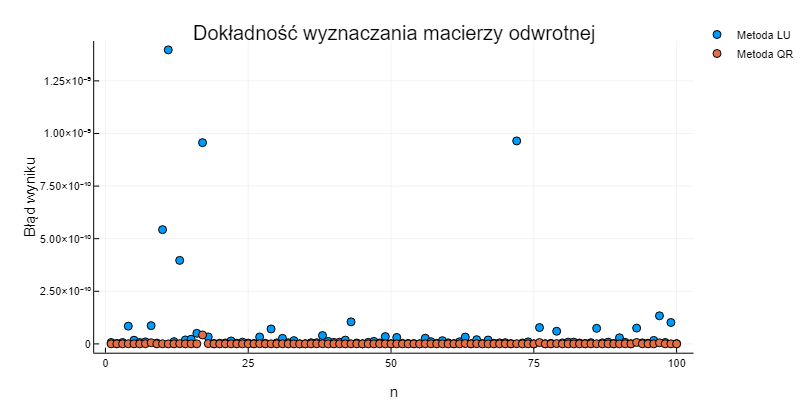
\includegraphics[scale=0.50]{wykres4.png}
\end{center}
Jak widać z wykresu dla macierzy tego typu metoda oparta na rozkładzie $QR$ jest dokładniejsza oraz stabilniejsza od metody opartej na rozkładzie $LU$. Błąd wyznaczenia $A^{-1}$ za pomocą metody $QR$ nie przekracza $1 \cdot 10^{-12}$ podczas gdy błąd dla metody $LU$ dla niektórych macierzy przekracza wartość $1 \cdot 10^{-9}$. 

\paragraph{Macierz $A$ z dominującą przekątną}

Rozważmy $100$ macierzy $A$ rozmiaru $100 \times 100$ z coraz mocniej dominującą przekątną. Niech dla $n=1$ macierz $A$ będzie macierzą z losowymi wartościami całkowitymi z przedziału $[-50,50]$. Wraz ze wzrostem $n$ do wartości na przekątnej macierzy $A$ będziemy dodawać losowe wartości, by ostatecznie dla $n=100$ wartości na przekątnej macierzy $A$ były rzędu $1 \cdot 10^{6}$. Zbadamy dokładność wyznaczania $A^{-1}$ dla kolejnych tak zdefiniowanych macierzy $A$ za pomocą metod $LU$ oraz $QR$.

\begin{center}
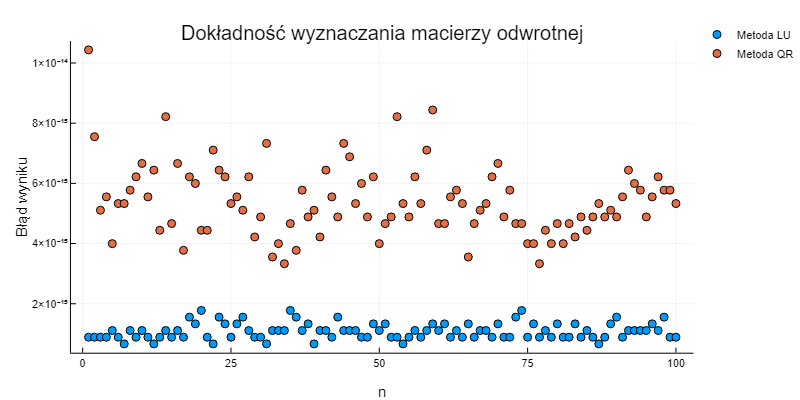
\includegraphics[scale=0.50]{wykres1.png}
\end{center}
Z wykresu wynika, że dla macierzy $A$ tego typu obie metody mają dobrą dokładność, lecz to metoda oparta na rozkładzie $LU$ jest lepsza. Dokładności obu metod są jednak tego samego rzędu, wiec różnica nie jest wyraźna. 

\paragraph{Macierz $A = Q^{T} \cdot B \cdot Q$}
Rozważmy $100$ macierzy $A$ rozmiaru $A$ rozmiaru $100 \times 100$. Niech $Q$ będzie pewną macierzą ortogonalną tego samego rozmiaru. Wówczas niech:

\begin{center}
\begin{math}
A = Q^{T} \cdot
\begin{bmatrix}
    \lambda_{11} & 0 & \dots  & 0 \\
    0 & \lambda_{22} & \dots  & 0 \\
    \vdots & \vdots & \ddots & \vdots \\
    0 & 0 & \dots  & \lambda_{nn}
\end{bmatrix}
\cdot Q
\end{math}
\end{center}
Niech dla każdej macierzy $A$ zachodzi własność $\lambda_{11} \geq \lambda_{22} \geq ... \geq \lambda_{nn}$ oraz niech wartości lambda będą początkowo zbliżone (dla $n=1$ spełniona jest własność $\lambda_{11} \sim \lambda_{22} \sim ... \sim \lambda_{nn} $), a następnie niech wartości $\lambda$ rosną, stając się do siebie coraz mocniej różne. Porównamy dokładność wyznaczania macierzy $A^{-1}$ za pomocą metod $LU$ oraz $QR$ dla tak zdefiniowanych macierzy $A$.

\begin{center}
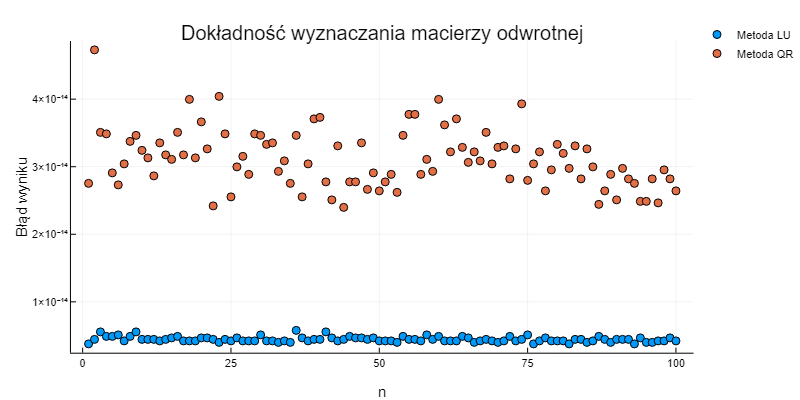
\includegraphics[scale=0.50]{wykres2.png}
\end{center}
Z wykresu wynika, że w przypadku macierzy $A$ tego typu metoda $LU$ okazuje się ponownie dokładniejsza od metody $QR$. Błąd dokładności metody opartej na rozkładzie $QR$ jest rzędu $1 \cdot 10^{-14}$, a metody opartej na rozkładzie $LU$ jest rzędu $1 \cdot 10^{-15}$. Warto zaznaczyć, że pomimo różnicy jednego rzędu dokładności, to obie metody mają dobrą dokładność.

\subsection{Poprawność numeryczna metod LU oraz QR}

Rozważmy macierz $A$ oraz $\overline{A}$ takie, że $\overline{a_{ij}} = a_{ij} + \epsilon$, gdzie $\epsilon \in (-10^{-13},10^{-13})$. Porównamy wartości $ \|  A^{-1} - \overline{A}^{-1} \| $, jeśli badana metoda jest numerycznie poprawna wartość ta powinna nie przekraczać $1 \cdot 10^{-13}$.
Zbadajmy 100 macierzy $A$ rozmiaru $25 \times 25$, których elementy to losowe liczby całkowite z przedziału $[-50,50]$. Na ich podstawie zbadamy poprawność numeryczną metod $QR$ oraz $LU$ w sposób opisany powyżej.

\begin{center}
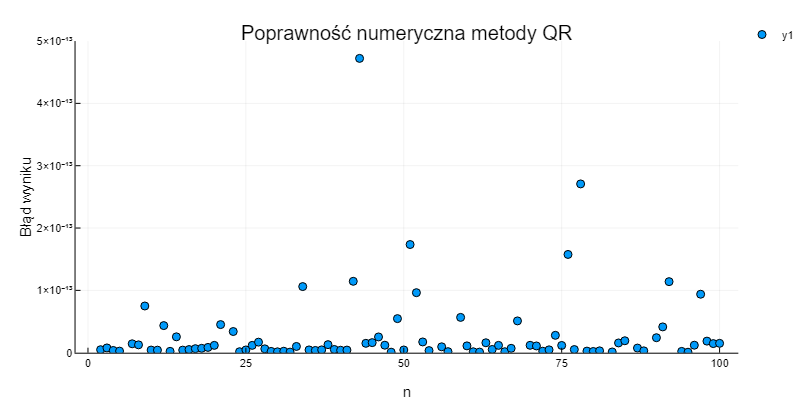
\includegraphics[scale=0.50]{wykres3.png}
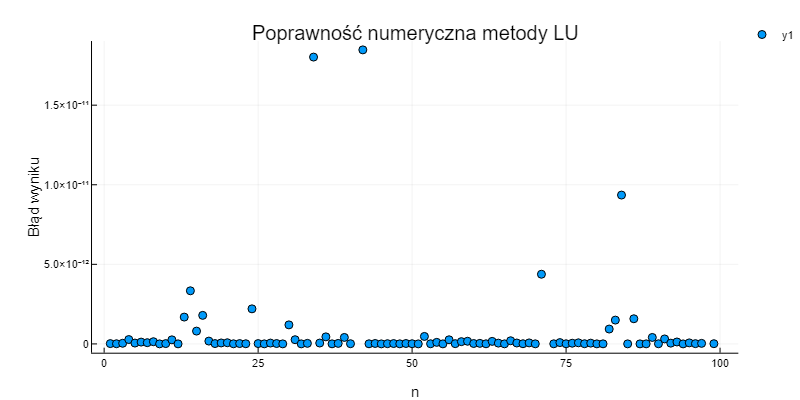
\includegraphics[scale=0.50]{wykres5.png}
\end{center}
Z wykresów widzimy, że metoda $QR$ jest bardziej poprawna numerycznie od metody $LU$. Dla większości macierzy błąd uzyskanego wyniku jest niewielki, jednak w przypadku metody $LU$ zdarzają się macierze, dla których wartość $ \|  A^{-1} - \overline{A}^{-1} \| $ jest rzędu $1 \cdot 10^{-9}$, co nie zdarza się w przypadku metody $QR$.

\subsection{Wnioski}

Z przeprowadzonych obliczeń wynika, że metoda znajdowania $A^{-1}$ oparta na rozkładzie $QR$ jest bardziej stabilna i numerycznie poprawna od metody opartej na rozkładzie $LU$, chociaż dla pewnych grup macierzy jest mniej dokładna (lecz nadal uzyskiwany błąd jest akceptowalny w zdecydowanej większości przypadków). Warto również zauważyć, że znając rozkłady $QR$ oraz $LU$ danej macierzy $A$ wyznaczenie $A^{-1}$ na podstawie rozkładu $QR$ jest o wiele prostsze oraz numerycznie poprawne od wyznaczania macierzy odwrotnej na podstawie rozkładu $LU$. Na wyniki wpływ ma więc to, że sam proces znajdowania rozkładu $QR$ powoduje większe błędy numeryczne od procesu znajdowania rozkładu $LU$. Powyższa obserwacja potwierdza się również w przypadku funkcji bibliotecznych z pakietu ,,Linear Algebra''. 

\section{Podsumowanie}

Wyznaczenie macierzy odwrotnej do danej macierzy $A$ za pomocą rozkładu $QR$ jest metodą gwarantującą stabilność, numeryczną poprawność oraz zadowalającą dokładność. Pomimo, że istnieją macierze, dla których wyznaczenie $A^{-1}$ za pomocą rozkładu $LU$ jest dokładniejsze, niż wyznaczenie macierzy odwrotnej za pomocą rozkładu $QR$, metoda $QR$ gwarantuje nam większą stabilność i pewność uzyskanego wyniku. Należy być jednak świadomym faktu, że obie te metody posiadają swoje wady i zalety.

\section{Literatura}

1) D. Kincaid, W. Cheney, Analiza numeryczna, WNT, 2005.\\
2) A. Schegel (aaronsc32), QR Decomposition with Householder Reflections, RPubs, 2018.\\
3) Mathematics Source Library C\&ASM, mymathlib.com, 2004.\\
4) D. Bindel, Matrix Computations (CS6210), Cornell University, Sep 28 2012.\\ 


	 

\end{document}
